%Este trabalho está licenciado sob a Licença Creative Commons Atribuição-CompartilhaIgual 3.0 Não Adaptada. Para ver uma cópia desta licença, visite https://creativecommons.org/licenses/by-sa/3.0/ ou envie uma carta para Creative Commons, PO Box 1866, Mountain View, CA 94042, USA.
% !TEX root = ../main.tex
\chapter{A propriedade de linearidade e a transformada da derivada}
\section{Linearidade da transformada de Laplace}
\begin{teo}{\label{prop_lin}}(Propriedade da linearidade)
A transformada de Laplace é uma transformação linear, isto é,
\begin{equation}
\mathcal{L }\left\{\alpha f(t)+\beta g(t)\right\}=\alpha \mathcal{L }\left\{ f(t)\right\}+\beta\mathcal{L }\left\{g(t)\right\}
\end{equation}
sempre que cada uma das transformadas existirem.
\end{teo}
\begin{proof}
Isso vem direto da propriedade de linearidade da integral:
\begin{eqnarray*}
\mathcal{L }\left\{\alpha f(t)+\beta g(t)\right\}&=&\int_0^\infty \left(\alpha f(t)+\beta g(t)\right)e^{-st}dt\\
&=&\int_0^\infty \alpha f(t)e^{-st}dt+\int_0^\infty\beta g(t)e^{-st}dt\\
&=&\alpha\int_0^\infty  f(t)e^{-st}dt+\beta\int_0^\infty g(t)e^{-st}dt\\
&=&\alpha \mathcal{L }\left\{ f(t)\right\}+\beta\mathcal{L }\left\{g(t)\right\}.
\end{eqnarray*}
\end{proof}
\begin{ex}{\label{ex_trans_sin_2}} A transformada de Laplace da função $f(t)=\sen(wt)$ já foi calculada no exemplo \ref{ex_trans_sin}. Agora vamos calcular novamente usando o resultado do exemplo \ref{ex_trans_exp} e a linearidade da transformada de Laplace. Primeiro recordamos a fórmula de Euler para escrever exponenciais complexas em termos de senos e cossenos:
\begin{eqnarray*}
e^{iwt}&=&\cos(wt)+i\sen(wt)\\
&\hbox{ou}&\\
e^{-iwt}&=&\cos(wt)-i\sen(wt) .
\end{eqnarray*}
As duas expressões podem ser resolvidas em termos do seno e do cosseno para obter
\begin{eqnarray}
{\label{ex_sen}} \sen(wt)&=&\frac{e^{iwt}-e^{-iwt}}{2i}\\
{\label{ex_cos}} \cos(wt)&=&\frac{e^{iwt}+e^{-iwt}}{2}
\end{eqnarray}
Agora podemos calcular a transformada de Laplace do seno usando a expressão (\ref{ex_sen}).
\begin{eqnarray*}
\mathcal{L }\{\sen(wt)\}&=&\mathcal{L }\left\{\frac{e^{iwt}-e^{-iwt}}{2i}\right\}\\
&=&\frac{1}{2i} \mathcal{L }\left\{ e^{iwt}\right\}-\frac{1}{2i} \mathcal{L }\left\{ e^{-iwt}\right\}\\
&=&\frac{1}{2i}\left( \frac{1}{s-iw}- \frac{1}{s+iw}\right)\\
&=&\frac{1}{2i}\left( \frac{s+iw-(s-iw)}{(s-iw)(s+iw)}\right)\\
&=&\frac{1}{2i}\left( \frac{2iw}{s^2+w^2}\right)\\
&=&\frac{w}{s^2+w^2}
\end{eqnarray*}
\end{ex}
\begin{ex} A transformada de Laplace da função $f(t)=\senh(wt)$ pode ser calculada usando o resultado do exemplo \ref{ex_trans_exp} e as expressões em termos de exponenciais:
\begin{eqnarray}
{\label{ex_senh}} \senh(at)&=&\frac{e^{at}-e^{-at}}{2}\\
{\label{ex_cosh}} \cosh(at)&=&\frac{e^{at}+e^{-at}}{2}.
\end{eqnarray}
Aplicamos a propriedade \ref{prop_lin} a expressão (\ref{ex_senh}) e temos:
\begin{eqnarray*}
\mathcal{L }\{\senh(at)\}&=&\mathcal{L }\left\{\frac{e^{at}-e^{-at}}{2}\right\}\\
&=&\frac{1}{2} \mathcal{L }\left\{ e^{at}\right\}-\frac{1}{2} \mathcal{L }\left\{ e^{-at}\right\}\\
&=&\frac{1}{2}\left( \frac{1}{s-a}- \frac{1}{s+a}\right)\\
&=&\frac{1}{2}\left( \frac{s+a-(s-a)}{(s-a)(s+a)}\right)\\
&=&\frac{1}{2}\left( \frac{2a}{s^2-a^2}\right)\\
&=&\frac{a}{s^2-a^2}
\end{eqnarray*}
\end{ex}
\begin{ex}Vamos calcular a tranformada de Laplace da função $f(t)=wt-\sen(wt)$ usando propriedade de linearidade \ref{prop_lin} e o exemplo \ref{ex_trans_sin_2}:
\begin{eqnarray*}
\mathcal{L }\{wt-\sen(wt)\}&=& w\mathcal{L }\left\{ t\right\}- \mathcal{L }\left\{ \sen(wt)\right\}\\
&=&\frac{w}{s^2}-\frac{w}{s^2+w^2}\\
&=&\frac{w(s^2+w^2)-ws^2}{s^2(s^2+w^2)}\\
&=&\frac{w(s^2+w^2)-ws^2}{s^2(s^2+w^2)}=\frac{w^3}{s^2(s^2+w^2)}\\
\end{eqnarray*}
\end{ex}
\begin{obs}A transformada inversa de Laplace também é uma transformação linear, isto é,
\begin{equation}{\label{prop_lin_inv}}
\mathcal{L }^{-1}\left\{\alpha F(s)+\beta G(s)\right\}=\alpha f(t)+\beta g(t).
\end{equation}
Esse resultado é consequência da propriedade de linearidade \ref{prop_lin}:
\begin{eqnarray*}
\mathcal{L }^{-1}\left\{\alpha F(s)+\beta G(s)\right\}&=&\mathcal{L }^{-1}\left\{\alpha \mathcal{L}\{f(t)\}+\beta \mathcal{L}\{g(t)\}\right\}\\
&=&\mathcal{L }^{-1}\left\{\mathcal{L}\left\{\alpha f(t)+\beta g(t)\right\}\right\}\\
&=&\alpha  f(t)+\beta g(t).
\end{eqnarray*}
\end{obs}
\begin{ex}Vamos calcular a tranformada inversa de Laplace da função $F(s)=\frac{2}{s}+\frac{4}{s^2}-\frac{1}{s-1}$ usando propriedade de linearidade \ref{prop_lin_inv} e a tabela \ref{tab_1}:
\begin{eqnarray*}
\mathcal{L }^{-1}\left\{\frac{2}{s}+\frac{4}{s^2}-\frac{1}{s-1}\right\}&=& 2\mathcal{L }^{-1}\left\{\frac{1}{s}\right\}+4\mathcal{L }^{-1}\left\{\frac{1}{s^2}\right\}-\mathcal{L }^{-1}\left\{\frac{1}{s-1}\right\}\\
&=&2+4t-e^t
\end{eqnarray*}
\end{ex}

\subsection*{Exercícios}
\begin{exer} Use a propriedade de linearidade \ref{prop_lin} para calcular a transformada de Laplace das seguintesfunções
 \begin{itemize}
  \item[a)] $f(t)=-8t+2\sen(5t)$
  \item[b)] $f(t)=-3t^2(t-2)$
  \item[c)] $f(t)=(2t-3)^3$
  \item[d)] $f(t)=\cos(t)^2$
  \item[f)] $f(t)=\sen(t)^3$
  \item[g)] $f(t)=\cosh(t)^3$
 \item[h)] $f(t)=\cos(wt)$.
 \item[i)] $f(t)=e^{at}-e^{bt}$.
 \item[j)] $f(t)=\cosh(at)$.
 \item[k)] $f(t)=1-\cos(wt)$.
  \end{itemize}
 \end{exer}
\begin{resp}
 \begin{itemize}
  \item[a)] $F(s)=-\frac{8}{s^2}+\frac{10}{s^2+25}$
  \item[b)] $F(s)=-\frac{18}{s^4}+\frac{12}{s^3}$
  \item[c)] $F(s)=\frac{48}{s^4}-\frac{72}{s^3}+\frac{54}{s^2}-\frac{27}{s}$
  \item[d)] $F(s)=\frac{s^2+2}{s^3+4s}$
  \item[e)] $F(s)=\frac{6}{s^4+10s^2+9}$
  \item[f)] $F(s)=\frac{s(s^2-7)}{s^4-10s^2+9}$
 \end{itemize}
\end{resp}
\begin{exer} Use a linearidade da transformada inversa para calcular a transformada inversa de Laplace das seguintes funções
 \begin{itemize}
  \item[a)] $F(s)=\frac{2s-8}{s^2+4}$
  \item[b)] $F(s)=2s\left(\frac{1}{s^2-4}+\frac{1}{s(s^2-4)}\right)$
 \end{itemize}
 \end{exer}
\begin{resp}
 \begin{itemize}
  \item[a)] $f(t)=2\cos(2t)-4\sen(2t)$
  \item[b)] $f(t)=2\cosh(2t)+\senh(2t)$
 \end{itemize}
\end{resp}
\begin{exer}Resolva os seguintes itens
\begin{itemize}
 \item[a)] Use a definição para mostrar que $\mathcal{L}\{e^{zt}\}=\frac{1}{s-z}$, $z\in\mathbb{C}$.
 \item[b)] Use a fórmula do item a) para concluir que
 \begin{equation}
 \mathcal{L}\{e^{(a+ib)t}\}=\frac{s-a+ib}{(s-a)^2+b^2}
 \end{equation}
 \item[c)] Use a fórmula de Euler e o item b) para concluir que
  \begin{equation}
 \mathcal{L}\{e^{at}\cos(bt)\}=\frac{s-a}{(s-a)^2+b^2}
 \end{equation}
 e
  \begin{equation}
 \mathcal{L}\{e^{at}\sen(bt)\}=\frac{b}{(s-a)^2+b^2}
 \end{equation}
\end{itemize}
\end{exer}
\section{A transformada de Laplace da derivada de uma função}
\begin{teo}{\label{prop_der}}(Propriedade da transformada da derivada) Se $f(t)$ é contínua e de ordem exponencial e $f'(t)$ é contínua por partes para $t\geq 0$, então
\begin{equation}{\label{prop_der_1}}
\mathcal{L }\{f'(t)\}=s \mathcal{L }\{ f(t)\}-f(0).
\end{equation}
\end{teo}
\begin{proof}
Primeiro considere $f(t)$ e $f'(t)$ contínuas nos reais não negativos. Usando integração por partes na definição de transformada de Laplace, temos
\begin{eqnarray*}
 \mathcal{L}\{f'(t)\}&=&\int_0^\infty e^{-st} f'(t)dt\\
 &=&\left.e^{-st}f(t)\right|_0^\infty-  \int_0^\infty (-se^{-st}) f(t)dt\\
 &=&-f(0)+  s\int_0^\infty e^{-st}f(t)dt\\
 &=&-f(0)+  s\mathcal{L}\{f(t)\}
 \end{eqnarray*}
Se $f'(t)$ for contínua por partes, então separamos as integrais em somas de tal forma que $f'(t)$ seja contínua em cada parcela. Aplicamos integração por partes em cada parcela e obtemos o resultado desejado.
\end{proof}
Considere $f(t)$ e $f'(t)$ contínuas e $f''(t)$ contínua por partes. Então podemos aplicar a expressão \ref{prop_der_1} duas vezes e obter:
\begin{eqnarray}
\nonumber \mathcal{L }\{f''(t)\}&=&s \mathcal{L }\{ f'(t)\}-f'(0)\\
\nonumber &=&s\left( s \mathcal{L }\{ f(t)\}-f(0)\right)-f'(0)\\
&=& s^2 \mathcal{L }\{ f(t)\}-sf(0)-f'(0). {\label{prop_der_2}}
\end{eqnarray}
Analogamente, se $f(t),\ f'(t), \cdots, f^{(n-1)}(t)$ são contínuas e $f^{(n)}(t) $ é contínua por partes, então
\begin{eqnarray}{\label{prop_der_n}}
 \mathcal{L }\{f^{(n)}(t)\}= s^n \mathcal{L }\{ f(t)\}-s^{n-1}f(0)-s^{n-2}f'(0)-\cdots-f^{(n-1)}(0).
\end{eqnarray}
Vamos usar a propriedade \ref{prop_der} da transformada da derivada para calcular transformadas de Laplace.
\begin{ex}Vamos calcular a transformada de $f(t)=\cos(t)$ usando a propriedade \ref{prop_der}. Observe as derivadas:
  \begin{equation}
 f(t)=\cos(t),\qquad f'(t)=-\sen(t)\qquad\hbox{e}\qquad f''(t)=-\cos(t).
\end{equation}
Logo,
 \begin{equation}
f''(t)=-f(t).
\end{equation}
Aplicamos a transformada de Laplace e usamos a propriedade \ref{prop_der}:
 \begin{equation}
s^2F(s)-sf(0)-f'(0)=-F(s).
\end{equation}
Usamos o fato que $f(0)=\cos(0)=1$ e $f'(0)=-\sen(0)=0$ e obtemos
 \begin{equation}
s^2F(s)-s=-F(s),
\end{equation}
ou seja,
 \begin{equation}
F(s)=\frac{s}{s^2+1},
\end{equation}
que confere com o item 14 da tabela \ref{tab_trans_Lap_1}.
\end{ex}
\begin{ex}Agora, vamos calcular a transformada de $g(t)=t\cos(t)$ usando a propriedade \ref{prop_der} da transformada da derivada . Observe as derivadas:
 \begin{equation}
g'(t)=-t\sen(t)+\cos(t)
\end{equation}
e
 \begin{equation}
g''(t)=-t\cos(t)-\sen(t)-\sen(t),
\end{equation}
ou seja,
 \begin{equation}
g''(t)=-g(t)-2\sen(t).
\end{equation}
Aplicamos a transformada de Laplace e usamos a propriedade \ref{prop_der}:
 \begin{equation}
s^2G(s)-sg(0)-g'(0)=-G(s)-2\mathcal{L}\{\sen(t)\}.
\end{equation}
Usamos o fato que $g(0)=0\cdot\cos(0)=0$, $g'(0)=-0\cdot \sen(0)+\cos(0)=1$ e $\mathcal{L}\{\sen(t)\}=\frac{1}{s^2+1}$ e obtemos
 \begin{equation}
s^2G(s)-1=-G(s)-\frac{2}{s^2+1},
\end{equation}
isto é,
 \begin{equation}
G(s)=\frac{s^2-1}{(s^2+1)^2},
\end{equation}
\end{ex}

\subsection*{Exercícios}
\begin{exer}
Dado $f(t)=\cosh(at)$, sabemos que $f''(t)=a^2f(t)$, $f(0)=\cosh(0)=1$ e $f'(0)=a\sinh(0)=0$. Use essas informações e a propriedade da transformada da derivada para calcular $\mathcal{L}\{f(t)\}$.
\end{exer}
\begin{exer} Use a propriedade da transformada da derivada para calcular a transformada das seguintes funções:
\begin{center}

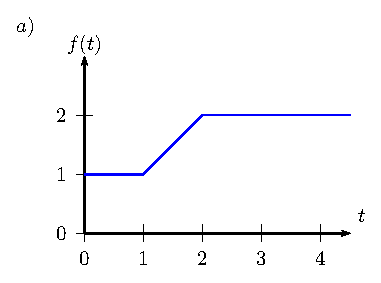
\includegraphics{cap_linear_deriva/pics/figura_1}
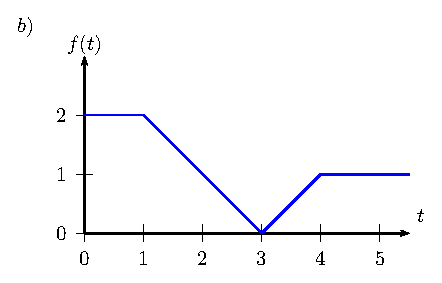
\includegraphics{cap_linear_deriva/pics/figura_2}\end{center}
\end{exer}
\begin{resp}
 \begin{itemize}
  \item[a)] $F(s)=\frac{1}{s}+\frac{e^{-s}-e^{-2s}}{s^2}$
      \item[b)] $F(s)=\frac{2}{s}+\frac{-e^{-s}+2e^{-3s}-e^{-4s}}{s^2}$
 \end{itemize}
\end{resp}
\section{Aplicação da transformada de Laplace para resolver problemas de valor inicial}
A propriedade da transformada da derivada \ref{prop_der}, juntamente com a propriedade da linearidade \ref{prop_lin}, são importantes para resolver problemas de valor inicial. A ideia é aplicar a transformada de Laplace à equação diferencial e, usando as condições iniciais escrevemos uma equação algébrica para transformada de Laplace da solução, que é chamada de {\bf equação subsidiária}. Em seguida, resolvemos a equação algébrica e calculamos a transformada inversa para obter a solução do problema. Por exemplo, considere o problema de valor inicial de segunda ordem
\begin{eqnarray*}
 y''(t)+ay'(t)+by(t)&=&f(t)\\
y(0)&=&y_0\\
y'(0)&=&y_0'
\end{eqnarray*}
com $a$, $b$, $y_0$ e $y_0'$ constantes. A aplicação da transformada de Laplace nos dá
 \begin{equation}
 \mathcal{L}\{y''(t)\}+a \mathcal{L}\{y'(t)\}+b \mathcal{L}\{y(t)\}= \mathcal{L}\{f(t)\}.
\end{equation}
Usando a propriedade \ref{prop_der}, obtemos a seguinte equação subsidiária
 \begin{equation}
 s^2\mathcal{L}\{y(t)\}-sy(0)-y'(0)+a s\mathcal{L}\{y(t)\}-ay(0)+b \mathcal{L}\{y(t)\}= \mathcal{L}\{f(t)\}
\end{equation}
ou seja,
 \begin{equation}
 Y(s)=\frac{F(s)+sy_0+y_0'+ay_0}{(s^2+as+b)}
\end{equation}
onde $\mathcal{L}\{y(t)\}=Y(s)$ e $\mathcal{L}\{f(t)\}=F(s)$. A solução do problema de valor inicial é  $y(t)=\mathcal{L}^{-1}\{Y(s)\}$.
\begin{ex}Vamos resolver o problema de valor inicial
\begin{eqnarray*}
 y''(t)+y(t)&=&2t\\
y(0)&=&2\\
y'(0)&=&1
\end{eqnarray*}
Primeiro aplicamos a transformada de Laplace na equação diferencial:
  \begin{equation}
 \mathcal{L}\{y''(t)\}+\mathcal{L}\{y(t)\}=\mathcal{L}\{2t\}
 \end{equation}
 Em seguida, usamos a equação \ref{prop_der_2} para obter
  \begin{equation}
s^2 \mathcal{L }\{ y(t)\}-sy(0)-y'(0)+\mathcal{L}\{y(t)\}=2\mathcal{L}\{t\}.
 \end{equation}
 Agora, usamos a notação $\mathcal{L }\{ y(t)\}=Y(s)$ e o fato que $\mathcal{L}\{t\}=\frac{1}{s^2}$ para escrever
  \begin{equation}
s^2 Y(s)-sy(0)-y'(0)+Y(s)=\frac{2}{s^2}.
 \end{equation}
 Obtemos a equação subsidiária quando substituímos $y(0)=2$ e $y'(0)=1$:
  \begin{equation}
s^2 Y(s)-2s-1+Y(s)=\frac{2}{s^2}.
 \end{equation}
 O próximo passo é resolver a equação algébrica para $Y(s)$
  \begin{equation}
 Y(s)\left(s^2+1\right)=\frac{2}{s^2}+2s+1,
 \end{equation}
 isto é,
  \begin{equation}
 Y(s)=\frac{2}{s^2\left(s^2+1\right)}+\frac{2s}{\left(s^2+1\right)}+\frac{1}{\left(s^2+1\right)}.
 \end{equation}
 A solução do problema de valor inicial pode ser escrita como
 \begin{equation}
y(t)=\mathcal{L}^{-1}\left\{\frac{2}{s^2\left(s^2+1\right)}\right\}+\mathcal{L}^{-1}\left\{\frac{2s}{\left(s^2+1\right)}\right\}+\mathcal{L}^{-1}\left\{\frac{1}{\left(s^2+1\right)}\right\}.
\end{equation}
 Obtemos as transformadas inversas olhando a tabela \ref{tab_trans_Lap_1} do apêndice \ref{ap_A}, itens 20, 14 e 13:
  \begin{equation}
 \mathcal{L}^{-1}\left\{\frac{1}{s^2\left(s^2+1\right)}\right\}=t-\sen(t),\qquad w=1\ \hbox{no item 20 da tabela \ref{tab_trans_Lap_1}}, \end{equation}
  \begin{equation}
 \mathcal{L}^{-1}\left\{\frac{s}{\left(s^2+1\right)}\right\}=\cos(t),\qquad w=1\ \hbox{no item 14 da tabela \ref{tab_trans_Lap_1}}
 \end{equation}
 e
  \begin{equation}
 \mathcal{L}^{-1}\left\{\frac{1}{\left(s^2+1\right)}\right\}=\sen(t),\qquad w=1\ \hbox{no item 13 da tabela \ref{tab_trans_Lap_1}}
 \end{equation}
 Combinando a propriedade da linearidade \ref{prop_lin}, temos:
  \begin{equation}
y(t)=2t-2\sen(t)+2\cos(t)+\sen(t)=2t+2\cos(t)-\sen(t)
\end{equation}
 \end{ex}
\begin{exer}Resolva o seguinte problema de valor inicial
\begin{eqnarray*}
 y''(t)+2y'(t)+y(t)&=&e^{-t}\\
y(0)&=&-1\\
y'(0)&=&1
\end{eqnarray*}
\end{exer}

\subsection*{Exercícios}
\begin{exer} Resolva os seguintes problemas de valor inicial
 \begin{itemize}
  \item[a)] $\displaystyle \left\{\begin{array}{l}y'+2y=1,\\ y(0)=3 \end{array}\right.$
    \item[b)] $\displaystyle \left\{\begin{array}{l}y'+3y=e^t,\\ y(0)=2 \end{array}\right.$
    \item[c)] $\displaystyle \left\{\begin{array}{l}y''+5y'+6y=0,\\ y(0)=1,\\ y'(0)=0 \end{array}\right.$
    \item[d)] $\displaystyle \left\{\begin{array}{l}y''+2y'+y=e^{-t},\\ y(0)=-1,\\ y'(0)=1 \end{array}\right.$
    \item[e)] $\displaystyle \left\{\begin{array}{l}y'' +  y = 2 \cos(t),\\ y(0)=3,\\ y'(0)=4 \end{array}\right.$
    \item[f)] $\displaystyle \left\{\begin{array}{l}y'' +7 y' +12 y = 21 e^{3t},\\ y(0)=3.5, \\ y'(0)=-10 \end{array}\right.$
 \end{itemize}
\end{exer}
\begin{resp}
 \begin{itemize}
  \item[a)] $y(t)=\frac{5}{2}e^{-2t}+\frac{1}{2}$
    \item[b)] $y(t)=\frac{1}{4}e^{t}+\frac{7}{4}e^{-3t}$
        \item[c)] $y(t)=3e^{-2t}-2e^{-3t}$
        \item[d)] $y(t)=\frac{1}{2}e^{-t}(t^2-2)$
        \item[e)] $y(t)= t \sen t + 3 \cos t +4 \sen t$
        \item[f)] $y(t)=\frac{e^{3t}}{2} + \frac{5e^{-4t}}{2} + \frac{e^{-3t}}{2}$
        \end{itemize}
\end{resp}



\section{Método das frações parciais para calcular transformadas inversas}
Suponha que $P(x)$ e $Q(x)$ são polinômios tais que o grau de $P$ é menor que o grau de $Q$. O polinômio $Q(x)$ pode ser fatorado em polinômios de graus um e dois:
 \begin{equation}
Q(x) = (a_1x + b_1)^{l_1}\cdots (a_nx + b_n)^{l_n}(c_1x^2 + d_1x + e_1)^{p_1}\cdots (c_m x^2 + d_m x + e_m)^{p_m}.
\end{equation}
Com isso, podemos encontrar constantes $A_{1,1}, \ldots, A_{n,l_1\cdots l_n}$, $B_{1,1}, \ldots, B_{m,p_1\cdots p_n}$ e $C_{1,1}, \ldots, C_{m,p_1\cdots p_n}$ tais que:
\begin{eqnarray*}
\frac{P(x)}{Q(x)} &=& \sum_{k=0}^{l_1-1} \frac{A_{1,k}}{(a_1x + b_1)^{l1-k}} + \cdots + \sum_{k=0}^{l_n-1}\frac{A_{n,k}}{(a_nx + b_n)^{l_n-k}} \\&+& \sum_{k=0}^{p_1-1} \frac{B_{1,k}x + C_{1,k}}{(c_1 x^2 + d_1 x + e_1)^{p_1-k}} + \cdots + \sum_{k=0}^{p_m-1} \frac{B_{m,k}x + C_{m,k}}{(c_mx^2 + d_mx + e_m)^{p_m-k}}.
\end{eqnarray*}
Esse método é usado para calcular integrais de funções racionais e transformadas inversas de Laplace.
\begin{ex}Para calcular a transformada inversa de Laplace da função racional $F(s)=\frac{1}{(s-1)(s^2-2s-5)}$ usamos o método de frações parciais, ou seja, encontramos $A$, $B$ e $C$ que satisfazem
\begin{eqnarray*}
 F(s)=\frac{1}{(s-1)(s^2+1)}&=&\frac{A}{s-1}+\frac{B+Cs}{s^2+1}\\&=&\frac{A(s^2+1)+(B+Cs)(s-1)}{(s-1)(s^2+1)}\\
 &=&\frac{s^2(A+C)+s(B-C)+A-B}{(s-1)(s^2+1)}.
\end{eqnarray*}
Obtemos o sistema
\begin{eqnarray*}
A+C&=&0\\
B-C&=&0\\
A-B&=&1
\end{eqnarray*}
que tem solução $B=C=-\frac{1}{2}$ e $A=\frac{1}{2}$. Logo,
 \begin{equation}
F(s)=\frac{1}{2}\left(\frac{1}{s-1}-\frac{s+1}{s^2+1}\right).
\end{equation}
Escrevendo em uma forma conveniente, temos
 \begin{equation}
F(s)=\frac{1}{2}\left(\frac{1}{s-1}-\frac{s}{s^2+1}-\frac{1}{s^2+1}\right).
\end{equation}
A transformada inversa é
 \begin{equation}
f(t)=\frac{1}{2}\left(e^{t}-\cos(t)-\sen(t)\right).
\end{equation}
\end{ex}

\subsection*{Exercícios}
\begin{exer}{\label{frac_parciais}} Realize a expansão em frações parciais das seguintes funções racionais $F(s)$ e calcule as respectivas transformadas inversas $f(t)=\mathcal{L}^{-1}\{F(s)\}$.
\begin{itemize}
\item[a)]$F(s)=\frac{s^2-6s+4}{s^3-3s^2+2s}$
\item[b)]$F(s)=\frac{s^2+s-2}{(s+1)^3}$
\item[c)]$F(s)=\frac{s}{(s+1)^3}$
\item[d)]$F(s)=\frac{5s^2-15s-11}{(s+1)(s-2)^3}$
\item[e)]$F(s)=\frac{3s^2-2s-1}{(s-3)(s^2+1)}$
\item[f)]$F(s)=\frac{s^2+2s+3}{(s^2+2s+2)(s^2+2s+5)}$
\item[g)]$F(s)=\frac{1}{s^2(s-2)}$
\end{itemize}
\end{exer}
\begin{resp}
\begin{itemize}
 \item [a)]
 \begin{eqnarray*}
F(s)&=&\frac{s^2-6s+4}{s^3-3s^2+2s}=\frac{s^2-6s+4}{s(s^2-3s+2)}=\frac{s^2-6s+4}{s(s-1)(s-2)}=\frac{A}{s}+\frac{B}{s-1}+\frac{C}{s-2}
\end{eqnarray*}
\begin{eqnarray*}
A&=&\lim_{s\to 0}sF(s)=\lim_{s\to 0}\frac{s^2-6s+4}{(s-1)(s-2)}=\left.\frac{s^2-6s+4}{(s-1)(s-2)}\right|_{s=0}=2\\
B&=&\lim_{s\to 1}(s-1)F(s)=\lim_{s\to 1}\frac{s^2-6s+4}{s(s-2)}=\left.\frac{s^2-6s+4}{s(s-2)}\right|_{s=1}=1\\
C&=&\lim_{s\to 2}(s-2)F(s)=\lim_{s\to 2}\frac{s^2-6s+4}{s(s-1)}=\left.\frac{s^2-6s+4}{s(s-1)}\right|_{s=2}=-2\\
\end{eqnarray*}
\begin{eqnarray*}
\mathcal{L}^{-1}\left\{F(s)\right\}&=&\mathcal{L}^{-1}\left\{\frac{2}{s}+\frac{1}{s-1}-\frac{2}{s-2}\right\}\\
&=&2+e^{t}-2e^{2t},t>0
\end{eqnarray*}
 \item [b)]
\begin{eqnarray*}
F(s)&=&\frac{s^2+s-2}{(s+1)^3}=\frac{A}{(s+1)^3}+\frac{B}{(s+1)^2}+\frac{C}{(s+1)}
\end{eqnarray*}
\begin{eqnarray*}
A&=&\lim_{s\to -1}(s+1)^3F(s)=\lim_{s\to 1}(s^2+s-2)=\left.(s^2+s-2)\right|_{s=-1}=-2\\
\end{eqnarray*}
Conhecendo o valor de $A$, reduzimos o problema a
\begin{eqnarray*}
\frac{s^2+s-2}{(s+1)^3}+\frac{2}{(s+1)^3}=\frac{B}{(s+1)^2}+\frac{C}{(s+1)}
\end{eqnarray*}
Simplificando o lado da esquerda, temos:
\begin{eqnarray*}
\frac{s^2+s-2}{(s+1)^3}+\frac{2}{(s+1)^3}=\frac{s^2+s}{(s+1)^3}=\frac{s(s+1)}{(s+1)^3}=\frac{s}{(s+1)^2}
\end{eqnarray*}
\begin{eqnarray*}
B&=&\lim_{s\to -1}(s+1)^2\frac{s}{(s+1)^2}=-1\\
\end{eqnarray*}
Reduzimos mais uma vez o problema a
\begin{eqnarray*}
\frac{s}{(s+1)^2}+\frac{1}{(s+1)^2}=\frac{C}{s+1}
\end{eqnarray*}
Simplificando o lado da esquerda, temos:
\begin{eqnarray*}
\frac{s}{(s+1)^2}+\frac{1}{(s+1)^2}=\frac{s+1}{(s+1)^2}=\frac{1}{s+1}
\end{eqnarray*}
o que implica $C=1$. Portanto temos:
\begin{eqnarray*}
F(s)&=&\frac{s^2+s-2}{(s+1)^3}=-\frac{2}{(s+1)^3}-\frac{1}{(s+1)^2}+\frac{1}{(s+1)}
\end{eqnarray*}
e, assim,
\begin{eqnarray*}
f(t)&=&e^{-t}\left(-t^2-t+1\right)
\end{eqnarray*}
\item [c)]
\begin{eqnarray*}
F(s)&=&\frac{s}{(s+1)^3}=\frac{s+1}{(s+1)^3}-\frac{1}{(s+1)^3}=\frac{1}{(s+1)^2}-\frac{1}{(s+1)^3}
\end{eqnarray*}
\begin{eqnarray*}
f(t)&=&e^{-t}\left(t-\frac{t^2}{2}\right)
\end{eqnarray*}
 \item [d)]
\begin{eqnarray*}
F(s)&=&\frac{5s^2-15s-11}{(s+1)(s-2)^3}=\frac{A}{s+1}+\frac{B}{(s-2)^3}+\frac{C}{(s-2)^2}+\frac{D}{(s-2)}
\end{eqnarray*}
\begin{eqnarray*}
A&=&\lim_{s\to -1}(s+1)F(s)=-\frac{1}{3}\\
B&=&\lim_{s\to 2}(s-2)^3F(s)=-7\\
\end{eqnarray*}
Obtém-se também
\begin{eqnarray*}
C&=&4\\
D&=&\frac{1}{3}
\end{eqnarray*}
Portanto
 \begin{equation}f(t)=-\frac{1}{3}e^{-t}+\left(-\frac{7}{2}t^2+4t+\frac{1}{3}\right)e^{2t}\end{equation}
 \item [e)]
\begin{eqnarray*}
F(s)&=&\frac{3s^2-2s-1}{(s-3)(s^2+1)}=\frac{A}{s-3}+\frac{Bs+C}{s^2+1}
\end{eqnarray*}
\begin{eqnarray*}
A=\lim_{s\to 3}(s-3)F(s)=2\\
\end{eqnarray*}
\begin{eqnarray*}
Bs+C&=&\left(F(s)-\frac{A}{s-3}\right)(s^2+1)\\
&=&\left(\frac{3s^2-2s-1}{(s-3)(s^2+1)}-\frac{2}{s-3}\right)(s^2+1)\\
&=&\left(\frac{3s^2-2s-1-2(s^2+1)}{(s-3)(s^2+1)}\right)(s^2+1)\\
&=&\frac{s^2-2s-3}{(s-3)}=\frac{(s+1)(s-3)}{(s-3)}=s+1
\end{eqnarray*}
Assim, $B=C=1$ e temos
$f(t)=e^{3t}+\cos(t)+\sin(t)$
 \item [f)]
\begin{eqnarray*}
F(s)&=&\frac{s^2+2s+3}{(s^2+2s+2)(s^2+2s+5)}=\frac{As+B}{s^2+2s+2}+\frac{Cs+D}{s^2+2s+5}\\
&=&\frac{(As+B)(s^2+2s+5)+(Cs+D)(s^2+2s+2)}{(s^2+2s+2)(s^2+2s+5)}\\
&=&\frac{(A+C)s^3+(2A+2C+B+D)s^2+(5A+2D+2B+2C)s+(5B+2D)}{(s^2+2s+2)(s^2+2s+5)}\\
\end{eqnarray*}
Comparando coeficientes, temos:
\begin{eqnarray*}
A+C&=&0\\
2A+2C+B+D&=&1\\
5A+2D+2B+2C&=&2\\
5B+2D&=&3
\end{eqnarray*}
\begin{eqnarray*}
A&=&0  \\
B&=&\frac{1}{3}  \\
C&=& 0 \\
D&=&\frac{2}{3}
\end{eqnarray*}
\begin{eqnarray*}
F(s)&=&\frac{1}{3}\frac{1}{s^2+2s+2}+\frac{2}{3}\frac{1}{s^2+2s+5}\\
&=&\frac{1}{3}\frac{1}{(s+1)^2+1}+\frac{2}{3}\frac{1}{(s+1)^2+2^2}
\end{eqnarray*}
\begin{eqnarray*}
f(t)=\frac{1}{3}e^{-t}\left[\sin(t)+\sin(2t)\right]
\end{eqnarray*}
 \item [g)]
\begin{eqnarray*}
F(s)&=&\frac{1}{s^2(s-2)}=\frac{A}{s}+\frac{B}{s^2}+\frac{C}{s-2}
\end{eqnarray*}
\end{itemize}
\end{resp}
